\section{mo\-No\-Aspir\-Crit$<$ M $>$ Class Template Reference}
\label{classmo_no_aspir_crit}\index{moNoAspirCrit@{moNoAspirCrit}}
One of the possible aspiration criterion ({\bf mo\-Aspir\-Crit}{\rm (p.\,\pageref{classmo_aspir_crit})}).  


{\tt \#include $<$mo\-No\-Aspir\-Crit.h$>$}

Inheritance diagram for mo\-No\-Aspir\-Crit$<$ M $>$::\begin{figure}[H]
\begin{center}
\leavevmode
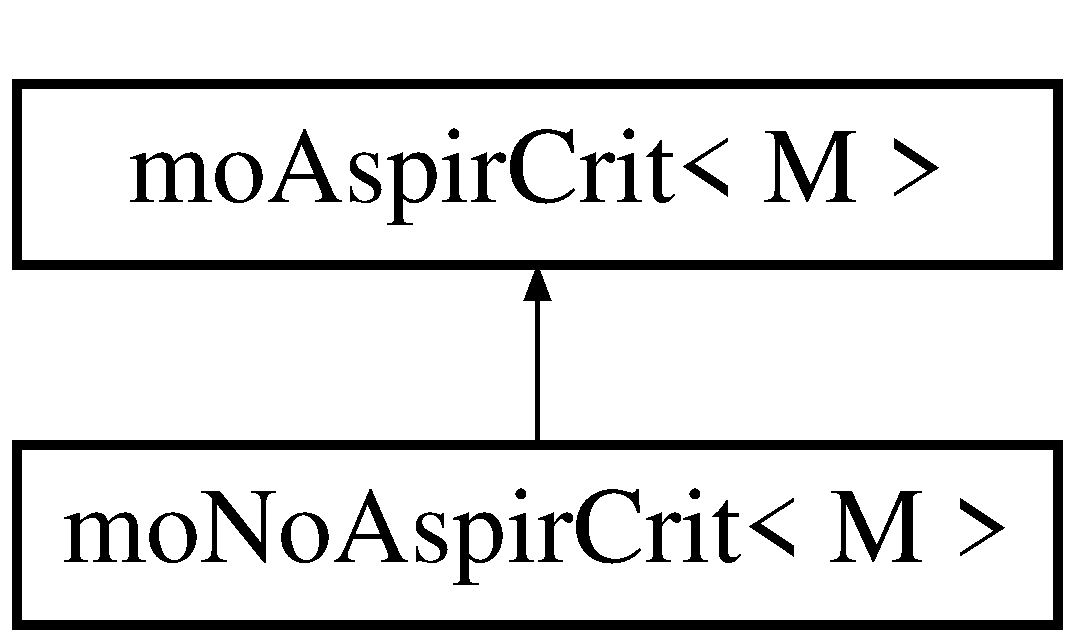
\includegraphics[height=2cm]{classmo_no_aspir_crit}
\end{center}
\end{figure}
\subsection*{Private Member Functions}
\begin{CompactItemize}
\item 
bool {\bf operator()} (const M \&\_\-\_\-move, const typename M::EOType::Fitness \&\_\-\_\-sol)
\begin{CompactList}\small\item\em Function which describes the aspiration criterion behaviour. \item\end{CompactList}\item 
void {\bf init} ()
\begin{CompactList}\small\item\em Procedure which initialises all that needs a {\bf mo\-No\-Aspir\-Crit}{\rm (p.\,\pageref{classmo_no_aspir_crit})}. \item\end{CompactList}\end{CompactItemize}


\subsection{Detailed Description}
\subsubsection*{template$<$class M$>$ class mo\-No\-Aspir\-Crit$<$ M $>$}

One of the possible aspiration criterion ({\bf mo\-Aspir\-Crit}{\rm (p.\,\pageref{classmo_aspir_crit})}). 

The simplest : never satisfied. 



Definition at line 21 of file mo\-No\-Aspir\-Crit.h.

\subsection{Member Function Documentation}
\index{moNoAspirCrit@{mo\-No\-Aspir\-Crit}!operator()@{operator()}}
\index{operator()@{operator()}!moNoAspirCrit@{mo\-No\-Aspir\-Crit}}
\subsubsection{\setlength{\rightskip}{0pt plus 5cm}template$<$class M$>$ bool {\bf mo\-No\-Aspir\-Crit}$<$ M $>$::operator() (const M \& {\em \_\-\_\-move}, const typename M::EOType::Fitness \& {\em \_\-\_\-sol})\hspace{0.3cm}{\tt  [inline, private]}}\label{classmo_no_aspir_crit_8a7180a8d5c25bfb6727d0b59551b0f8}


Function which describes the aspiration criterion behaviour. 

Does nothing.

\begin{Desc}
\item[Parameters:]
\begin{description}
\item[{\em \_\-\_\-move}]a move. \item[{\em \_\-\_\-sol}]a fitness. \end{description}
\end{Desc}
\begin{Desc}
\item[Returns:]FALSE. \end{Desc}


Definition at line 32 of file mo\-No\-Aspir\-Crit.h.\index{moNoAspirCrit@{mo\-No\-Aspir\-Crit}!init@{init}}
\index{init@{init}!moNoAspirCrit@{mo\-No\-Aspir\-Crit}}
\subsubsection{\setlength{\rightskip}{0pt plus 5cm}template$<$class M$>$ void {\bf mo\-No\-Aspir\-Crit}$<$ M $>$::init ()\hspace{0.3cm}{\tt  [inline, private, virtual]}}\label{classmo_no_aspir_crit_f3a286fc4c2d36bd390ba9a3074f3037}


Procedure which initialises all that needs a {\bf mo\-No\-Aspir\-Crit}{\rm (p.\,\pageref{classmo_no_aspir_crit})}. 

Nothing... 

Implements {\bf mo\-Aspir\-Crit$<$ M $>$} {\rm (p.\,\pageref{classmo_aspir_crit_a8ce84510a5ec7c9078381e542c6d140})}.

Definition at line 43 of file mo\-No\-Aspir\-Crit.h.

The documentation for this class was generated from the following file:\begin{CompactItemize}
\item 
mo\-No\-Aspir\-Crit.h\end{CompactItemize}
